\documentclass[a3paper]{article}
\usepackage{tikz}
\usepackage[margin=0in]{geometry}
\setlength{\parindent}{0mm}
\begin{document}

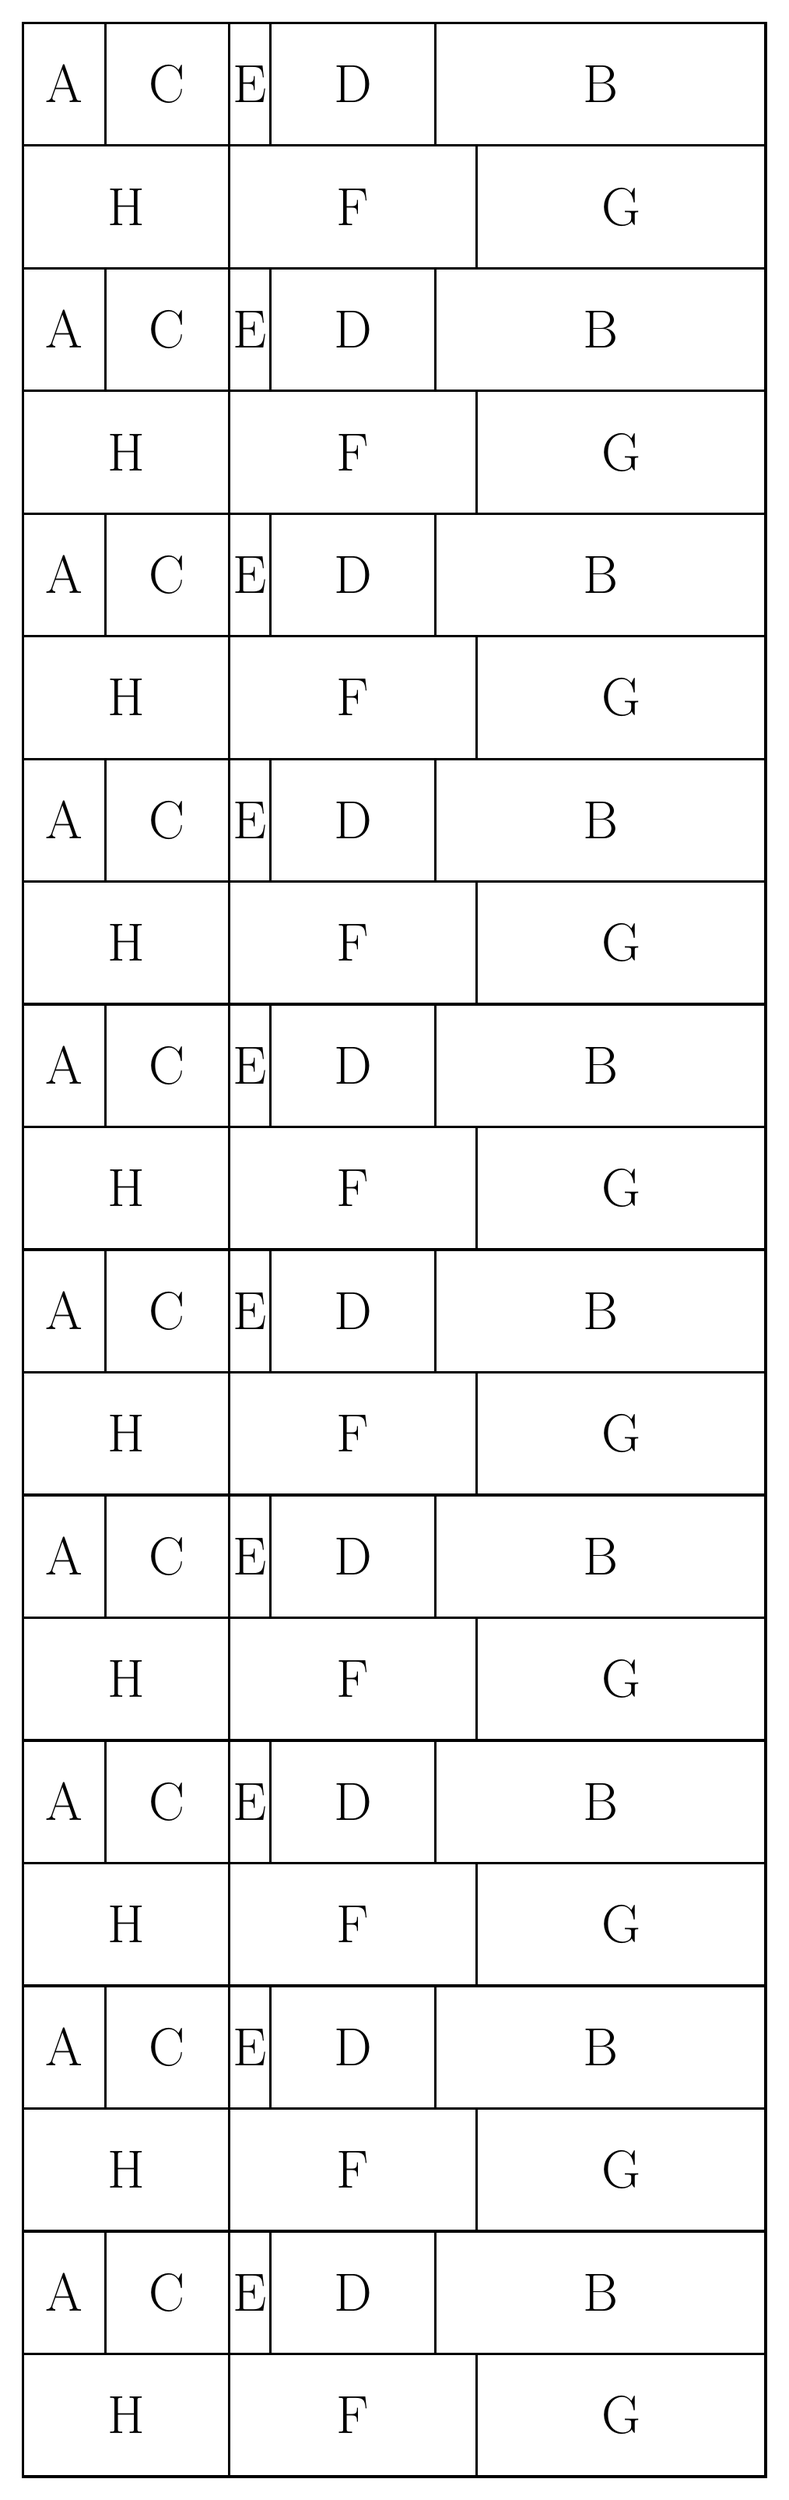
\begin{tikzpicture}
    \pgfmathsetmacro{\w}{2}	%width
    \newlength{\s}
    \pgfmathsetlength{\s}{\textwidth/18}	%scale
    \tikzset{
        sticks/.pic={
            \draw[very thick] (0,0) rectangle (2*\s,\w) node[midway] {\Huge A};
            \draw[very thick] (2*\s,0) rectangle ({5*\s},\w) node[midway] {\Huge C};
            \draw[very thick] ({5*\s},0) rectangle ({6*\s},\w) node[midway] {\Huge E};
            \draw[very thick] ({6*\s},0) rectangle ({10*\s},\w) node[midway] {\Huge D};
            \draw[very thick] (10*\s,0) rectangle (18*\s,\w) node[midway] {\Huge B};
            \draw[very thick] (0,0) rectangle (5*\s,-\w) node[midway] {\Huge H};
            \draw[very thick] ({5*\s},0) rectangle ({11*\s},-\w) node[midway] {\Huge F};
            \draw[very thick] (11*\s,0) rectangle (18*\s,-\w) node[midway] {\Huge G};}
    };
    \foreach \y in {0,1,...,9}{
        \draw (0,\y*\w*2) pic {sticks};
        % \draw (0,0) pic {sticks};
    }
\end{tikzpicture}

\end{document}